\appendices


\section{Complete Equation for the SABR model volatility}
\label{sec:sabr}

The SABR model is a stochastic volatility model developed as an extension of the Black-Scholes
model that allows for the volatility of the asset to be stochastic,
and is widely used in the financial industry for option pricing and risk management.
The implied volatility of the asset according to the model is given by the following equations~\cite{Hagan2002}:

\begin{equation*}
    \begin{aligned}
        F_t = S \cdot e^{(r - d)t}\\
        x(t) = \log \left( \frac{F_t}{K} \right)
    \end{aligned}
\end{equation*}
where $F_t$ is the price of a forward contract with the same underlying asset as the option,
$S$ is the spot price of the asset, $r$ the risk-free rate, and $d$ the dividend yield.
$x(t)$ is the log-moneyness value for the option.

\[
    y(t) = \left(F_t K\right)^{\frac{1 - \beta}{2}}
\]

\[
    z(t) = \frac{\nu}{\alpha}x(t) y(t)
\]

\[
    \kappa (t) = \log \left( \frac{\sqrt{1 - 2 \rho z(t) + z(t)^2} + z(t) - \rho}{1 - \rho} \right)
\]

where $y$ and $z$ are auxiliary functions to simplify the SABR model equation,
and $\kappa$ represents the adjustment factor for the volatility.

\[
    \sigma (t, K) = \alpha t
    \frac{
        \left( 1 + \left( \frac{(1 - \beta)^2 \alpha^2}{24 y(t)^2} + \frac{\alpha \beta \rho \nu }{4 y(t)} + \frac{(2 - 3 \rho^2) \nu^2}{24} \right) \right)
    } {
        \left( 1 + \frac{(1 - \beta)^2 x(t)^2}{24} + \frac{(1 - \beta)^4 x(t)^4}{1920} \right)
    } \frac{z(t)}{y(t)\kappa (t)}.
\]

Optimization for the $\alpha, \beta, \rho, \nu$ parameters is usually performed using constrained optimization methods,
and other algorithms such as adaptations of the Newton-Raphson method or Sequential Quadratic Programming can be used,
but choosing the best performing optimization method is outside the scope of this work.

\begin{figure*}
    \section{Interpolated Surfaces Comparison}
    \label{sec:surface_comparison}
    \centering
    % First row
    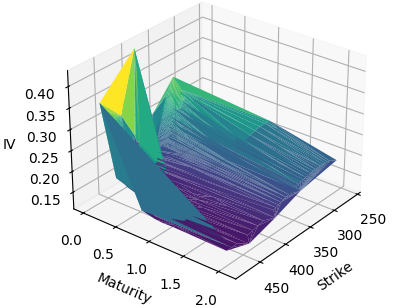
\includegraphics[width=6.5cm]{images/linear_1}
    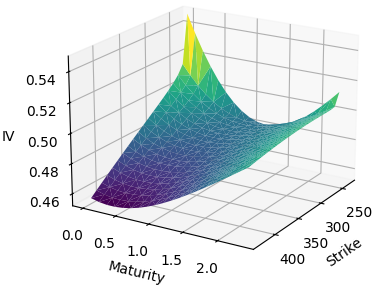
\includegraphics[width=6.5cm]{images/implicit_1}

    % Second row
    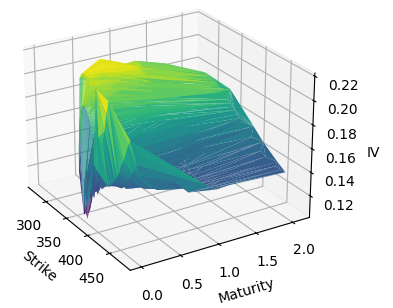
\includegraphics[width=6.5cm]{images/linear_2}
    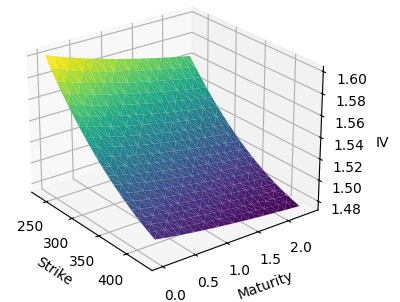
\includegraphics[width=6.5cm]{images/implicit_2}

    % Third row
    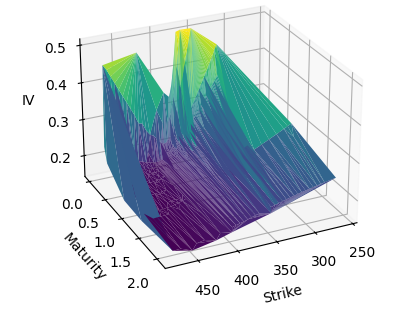
\includegraphics[width=6.5cm]{images/linear_3}
    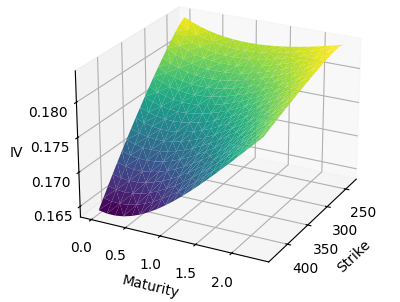
\includegraphics[width=6.5cm]{images/implicit_3}

    \caption{Surfaces interpolated on test data using a linear interpolation model (left) compared to the SABR models
    fitted with the candidate set selected using the trained implicit transformer architecture (right).}
    \label{fig:figure4}
\end{figure*}